% C3 load-shedding layers (build: pdflatex load-shedding-layers.tex -> load-shedding-layers.pdf)
\documentclass[tikz,border=4pt,11pt]{standalone}
\usepackage[T1]{fontenc}
\usepackage{lmodern}
\usetikzlibrary{shapes.geometric,positioning,fit,arrows.meta,backgrounds}
\begin{document}
\sffamily
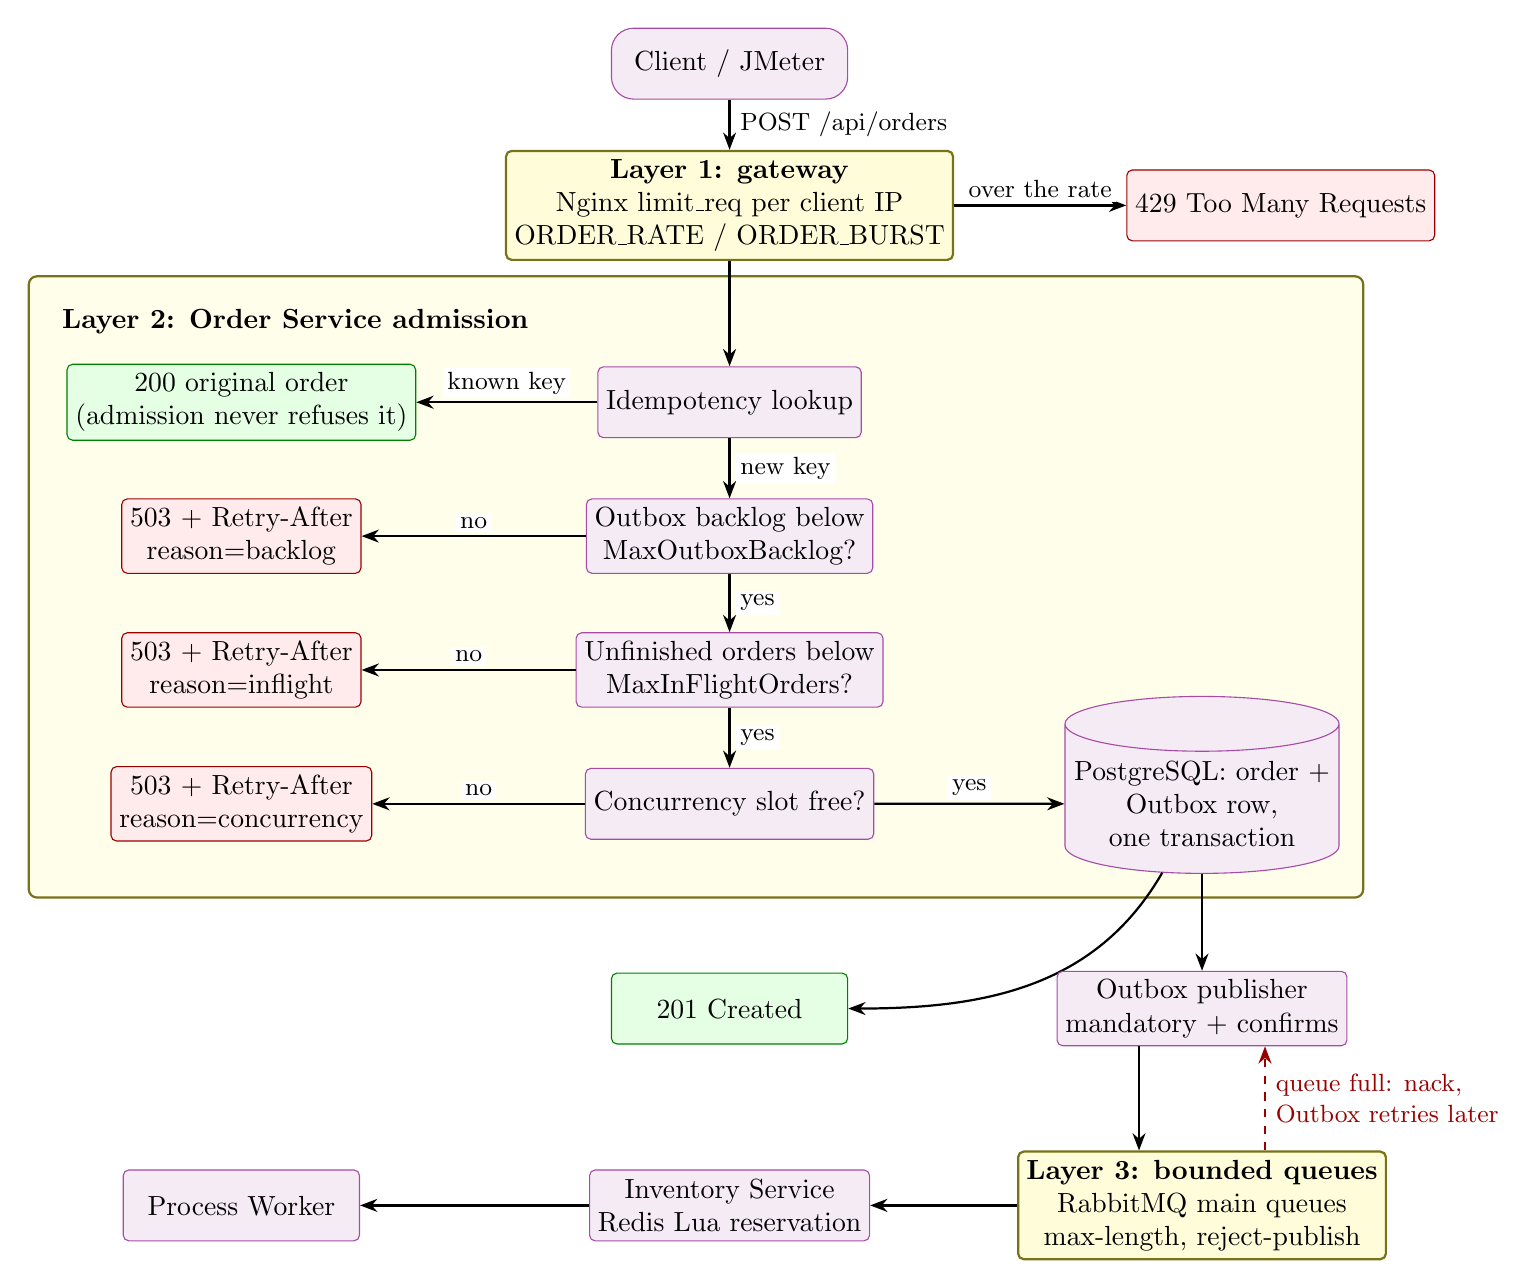
\begin{tikzpicture}[
  >={Stealth[length=2.2mm]},
  box/.style={draw=violet!70, fill=violet!8, rounded corners=2pt, align=center,
              minimum height=9mm, minimum width=30mm, inner sep=3pt},
  ok/.style={box, draw=green!50!black, fill=green!10},
  no/.style={box, draw=red!60!black, fill=red!8},
  layer/.style={box, draw=olive!80!black, fill=yellow!15, line width=0.8pt},
  db/.style={cylinder, shape border rotate=90, aspect=0.2, draw=violet!70,
             fill=violet!8, align=center, minimum width=30mm, minimum height=16mm},
  flow/.style={->, thick},
  lbl/.style={font=\small, fill=white, inner sep=1.5pt}
]
% entry and layer 1
\node[box, rounded corners=8pt] (c) at (5.6,0) {Client / JMeter};
\node[layer] (n) at (5.6,-1.8) {\textbf{Layer 1: gateway}\\Nginx limit\_req per client IP\\ORDER\_RATE / ORDER\_BURST};
\node[no] (r429) at (12.6,-1.8) {429 Too Many Requests};
\draw[flow] (c) -- node[lbl, right=2pt] {POST /api/orders} (n);
\draw[flow] (n) -- node[lbl, above=1pt] {over the rate} (r429);
% layer 2
\node[box] (i) at (5.6,-4.3) {Idempotency lookup};
\node[ok] (replay) at (-0.6,-4.3) {200 original order\\(admission never refuses it)};
\node[box] (b) at (5.6,-6.0) {Outbox backlog below\\MaxOutboxBacklog?};
\node[no] (r503b) at (-0.6,-6.0) {503 + Retry-After\\reason=backlog};
\node[box] (f) at (5.6,-7.7) {Unfinished orders below\\MaxInFlightOrders?};
\node[no] (r503f) at (-0.6,-7.7) {503 + Retry-After\\reason=inflight};
\node[box] (g) at (5.6,-9.4) {Concurrency slot free?};
\node[no] (r503c) at (-0.6,-9.4) {503 + Retry-After\\reason=concurrency};
\node[db] (w) at (11.6,-9.4) {PostgreSQL: order +\\Outbox row,\\one transaction};
\draw[flow] (n) -- (i);
\draw[flow] (i) -- node[lbl, above=1pt] {known key} (replay);
\draw[flow] (i) -- node[lbl, right=2pt] {new key} (b);
\draw[flow] (b) -- node[lbl, above=1pt] {no} (r503b);
\draw[flow] (b) -- node[lbl, right=2pt] {yes} (f);
\draw[flow] (f) -- node[lbl, above=1pt] {no} (r503f);
\draw[flow] (f) -- node[lbl, right=2pt] {yes} (g);
\draw[flow] (g) -- node[lbl, above=1pt] {no} (r503c);
\draw[flow] (g) -- node[lbl, above=1pt] {yes} (w);
\node[font=\bfseries, anchor=north west] (l2lbl) at (-3.0,-3.0) {Layer 2: Order Service admission};
\begin{scope}[on background layer]
  \node[draw=olive!80!black, fill=yellow!8, rounded corners=3pt, line width=0.8pt,
        fit=(l2lbl)(replay)(r503c)(w), inner sep=3mm] (l2) {};
\end{scope}
\node[ok] (created) at (5.6,-12.0) {201 Created};
\draw[flow] (w) to[out=-120,in=0] (created);
% publication and layer 3 (below layer 2, read right to left on the bottom row)
\node[box] (p) at (11.6,-12.0) {Outbox publisher\\mandatory + confirms};
\node[layer] (q) at (11.6,-14.5) {\textbf{Layer 3: bounded queues}\\RabbitMQ main queues\\max-length, reject-publish};
\node[box] (inv) at (5.6,-14.5) {Inventory Service\\Redis Lua reservation};
\node[box] (wk) at (-0.6,-14.5) {Process Worker};
\draw[flow] (w) -- (p);
\draw[flow] ([xshift=-8mm]p.south) -- ([xshift=-8mm]q.north);
\draw[flow, dashed, red!60!black] ([xshift=8mm]q.north) -- node[lbl, right=2pt, align=left] {queue full: nack,\\Outbox retries later} ([xshift=8mm]p.south);
\draw[flow] (q) -- (inv);
\draw[flow] (inv) -- (wk);
\end{tikzpicture}
\end{document}
